\documentclass{article}
\usepackage[utf8]{inputenc}
\usepackage{graphicx}
\graphicspath{ {images/} }
\usepackage{fullpage}
\linespread{1.5}

\title{Software Confinement Using Hardware-Assisted Virtualization}
\author{Yi-Fan Zhang}
\date{May 2016}

\newcommand{\PROJNAME}{\textit{hvexec}}

\begin{document}

\maketitle

\begin{abstract}
The ability to confine user-space software is critical for protecting users from
malicious or dubious application behavior.
With that in mind, we designed and implemented \PROJNAME{}, a virtualization layer that is interposed between applications and the kernel. Clients of \PROJNAME{} are given an API which they can use to monitor, filter or transform system calls from any application. To achieve this without requiring re-compiling or editing the application binary, we implemented \PROJNAME{} using an atypical application of hardware-assisted virtualization
where the restricted software executes in the context of a hardware virtual machine.
In this paper, we describe the benefits of using virtualization, the design and lessons learnt from our implementation and benchmarks to 
weight the benefits against the overhead.
\end{abstract}

\section{Introduction}
Local operating system security has traditionally focused on policing user interactions on multi-user systems \cite{DesignImplFreeBSD}.
However, in recent years, the pervasive use of personal computing along with the convenience of downloading
applications from the Internet has shifted the focus from restricting user privileges to limiting capabilites per application process
— sometimes referred to as sandboxing, application compartmentalization or process mitigation \cite{DesignImplFreeBSD}.
While conventional OS access controls based on notions such as users and groups have proven to be valuable,
they become awkward tools for applying security policy definitions on a per application basis \cite{DesignImplFreeBSD}.
Although numerous approaches to solve this particular problem have been proposed (see related works),
research into the best designs for applying sandboxing to software along with methods for decreasing overhead, remains active \cite{Ayer2012,VCall2010,DesignImplFreeBSD}.

In this paper, we propose \PROJNAME{}, an application sandbox designed to protect users from malicious or dubious application behavior.
To his end, we designed \PROJNAME{} against these principles:
\begin{itemize}
    \item \textbf{Resource Control:}
        Any access to system resources must be delegated through the sandbox.
    \item \textbf{Fidelity:}
        Applications must be loaded as native executables with no modifications to the binaries
        (no recompilation or binary translation) and behave equivalently as running outside the sandbox.
    \item \textbf{Flexibility:}
        Users should be given an API to program custom policies while the burden of enforcement falls upon the sandbox.
    \item \textbf{Performance:}
        Sandboxed applications should run as close as possible to unsandboxed speed
        and performance must not degrade significantly as more concurrent sandboxed processes are started.
    \item \textbf{Safety:}
        The sandbox must not weaken, circumvent or introduce new vulnerabilites into conventional OS access controls.
\end{itemize}
To help meet those requirements, our sandbox incorporates strategies from various related works.
At the foundation, we based \PROJNAME{} on an atypical application of hardware virtualization extensions (Intel VT-x) where
the sandboxed software (guest) executes in the context of a hardware virtual machine (HVM).
The hardware enforced nature of the virtual machine (VM) implicitly provides the advantage that the guest runs completely out-of-band with the host OS software.
By simulating a complete hardware environment within the VM, the guest has its own set of processor registers, physical memory and privilege modes.
More importantly, this requires the guest to cross a VM to host boundary before it can access any host resources
— similar to the hardware protection facilities provided for switching between user and kernel mode which is fundamental to implementing a reliable and secure operating system.
We exploit this property by dividing \PROJNAME{} into two parts: one runs as a user process on the host and another in kernel mode in the VM.
This assures that all guest system calls and accesses to privileged memory ranges can be trapped, and
by running \PROJNAME{} as an unprivileged user process on the host, we implicitly subject the
entire sandbox system to existing OS access control restrictions.
As part of the fedelity requirement, sandboxed applications must also not be able to detect the presence of the sandbox.
Otherwise, applications may choose to deny the user services in order to coerce permissions to be granted.

Aside from providing resiliance and isolation, \PROJNAME{} improves on prior work in terms of flexibility and performance.
In terms of flexibility, \PROJNAME{} exposes a user programmable API for defining security policies rather than a prescribed system wide security model commonly seen in previous approaches.
This returns control to the users while future proofing the system against the rapid changes in application development.
Furthermore, we mitigate the risk of introducing new system vulnerabilities by leveraging existing kernel support for virtualization hardware
such that no additional kernel modules need to be installed and no administrator privileges are needed to run \PROJNAME{}.
Although programs can execute natively within a VM, frequent context switching between VM and host can degrade performance.
We address this problem with a novel application of exitless notifications \cite{ELI2015} for VM and host communication that avoids
context switching entirely.

To validate our design, we provide an implementation of \PROJNAME{} built on OS X 10.11.4 — an operating system with
a rich set of user applications and kernel support for HVM.
For our evaluation, we weighed the benefits provided by \PROJNAME{} against the overhead using a suite of benchmarks on graphical and commandline applications as well as
microbenchmarks simulating worst case performance scenarios.
While the total virtualization overhead can be amortized over the total execution of the program \cite{Ayer2012, VCall2010}, the immediate affect on latency
sensitive applications has not been measured.
Similarily, the feasibility of scaling to hundreds of HVM sandboxed proccesses in is not known.
Thus, we also focused our investigation on aspects of scalability and context switching latency that were not previously examined.

In summary, we have proposed an application of hardware-assisted virtualization aimed at solving the problem of software confinement.
Our contributions include providing a user-programmable security system and a method of mitigating VM context switching latency.
Lastly, we believe the virtualization cost is well justified by the benefits attained, and we confirm our findings by benchmarks on \PROJNAME{} which we have also made open source.

The rest of the paper is organized as follows:
Section 2 compares \PROJNAME{} with related work.
Section 3 describes the design issues we faced and our solutions.
Section 4 presents benchmarks to evaluate \PROJNAME{}.
Section 5 suggests future direction and concludes the paper.

\section{Related Work}
In this section, we compare \PROJNAME{} with several representative works.
Our comparison does not imply that other approaches are not suitable for their original usage scenarios.
Instead, we intend to show that \PROJNAME{} improves on prior designs for addressing the requirements in the introduction section.

This is a sketch of what I want to cover:
\subsection{Kernel}

\begin{itemize}
    \item
        Directly modifying the kernel can achieve are the best performance and offers excellent assurances
    \item
        However, requires nontrivial code changes to kernel which has risk of introducing new vulnerabilities.
    \item
        Inconvenient for users; requires recompiling the kernel or permissions to install kernel extensions.
    \item
        Existing kernel features like ptrace are not suited for sandboxing (argument race conditions).
    \item
        Solutions like SELinux prescribe a fixed (non-programmable) security model.
    \item
        Shill Shell and Capsicum on FreeBSD provide programmable capability-based interface. However, the Shill Shell relies on FreeBSD's MAC framework which limits the granularity at which it can protect resources. Both do not support transformations on arguments and return values from system calls which are needed to implement virtual resources.
\end{itemize}

\subsection{Userspace}

\begin{itemize}
    \item
        Static binary translation is difficult on architectures with variable length instructions and jump targets not aligned to instruction boundaries.
    \item
        Does not handle JIT compiled programs.
    \item
        Dynamic binary translation requires complex runtime instruction decoding and tracing leads to poor performance.
    \item
        Application and security agent shares address space which makes it hard to ensure that application cannot override injected code.
    \item
        Custom loader/linker to interpose on system libraries is easily circumvented if program statically links dependencies or makes system calls directly.
    \item
        Managed runtime environments (Java) requires applications to be compiled with a specific toolchain (NaCl).
\end{itemize}

\subsection{Virtualization}
\begin{itemize}
    \item
        Full OS Virtualization is not scalable because of large overhead of running an entire guest operating system for each program.
    \item
        HVM is typically used in kernel virtualization but recently found use in less typical applications like malware analysis \cite{Ether2008} and sandboxing \cite{Ayer2012, VCall2010}.
    \item
        Most similar work include VCall and KVM sandbox to the best of our knowledge \cite{Ayer2012, VCall2010}.
    \item
        But they don't address scalability and both uses naive method of context switching that may not be suitable for low latency applications. Moreover, both use KVM on Linux. Instead, we want to do it on OSX, a more user-oriented OS.
\end{itemize}

\section{Design}
Describe design, optimizations and how to avoid pitfalls.
Explain how our design overcomes the limitations described in the related works section.
The only question remaining is the performance overhead of our approach which will be
addressed in the evaluation section.
\begin{figure}[ht]
    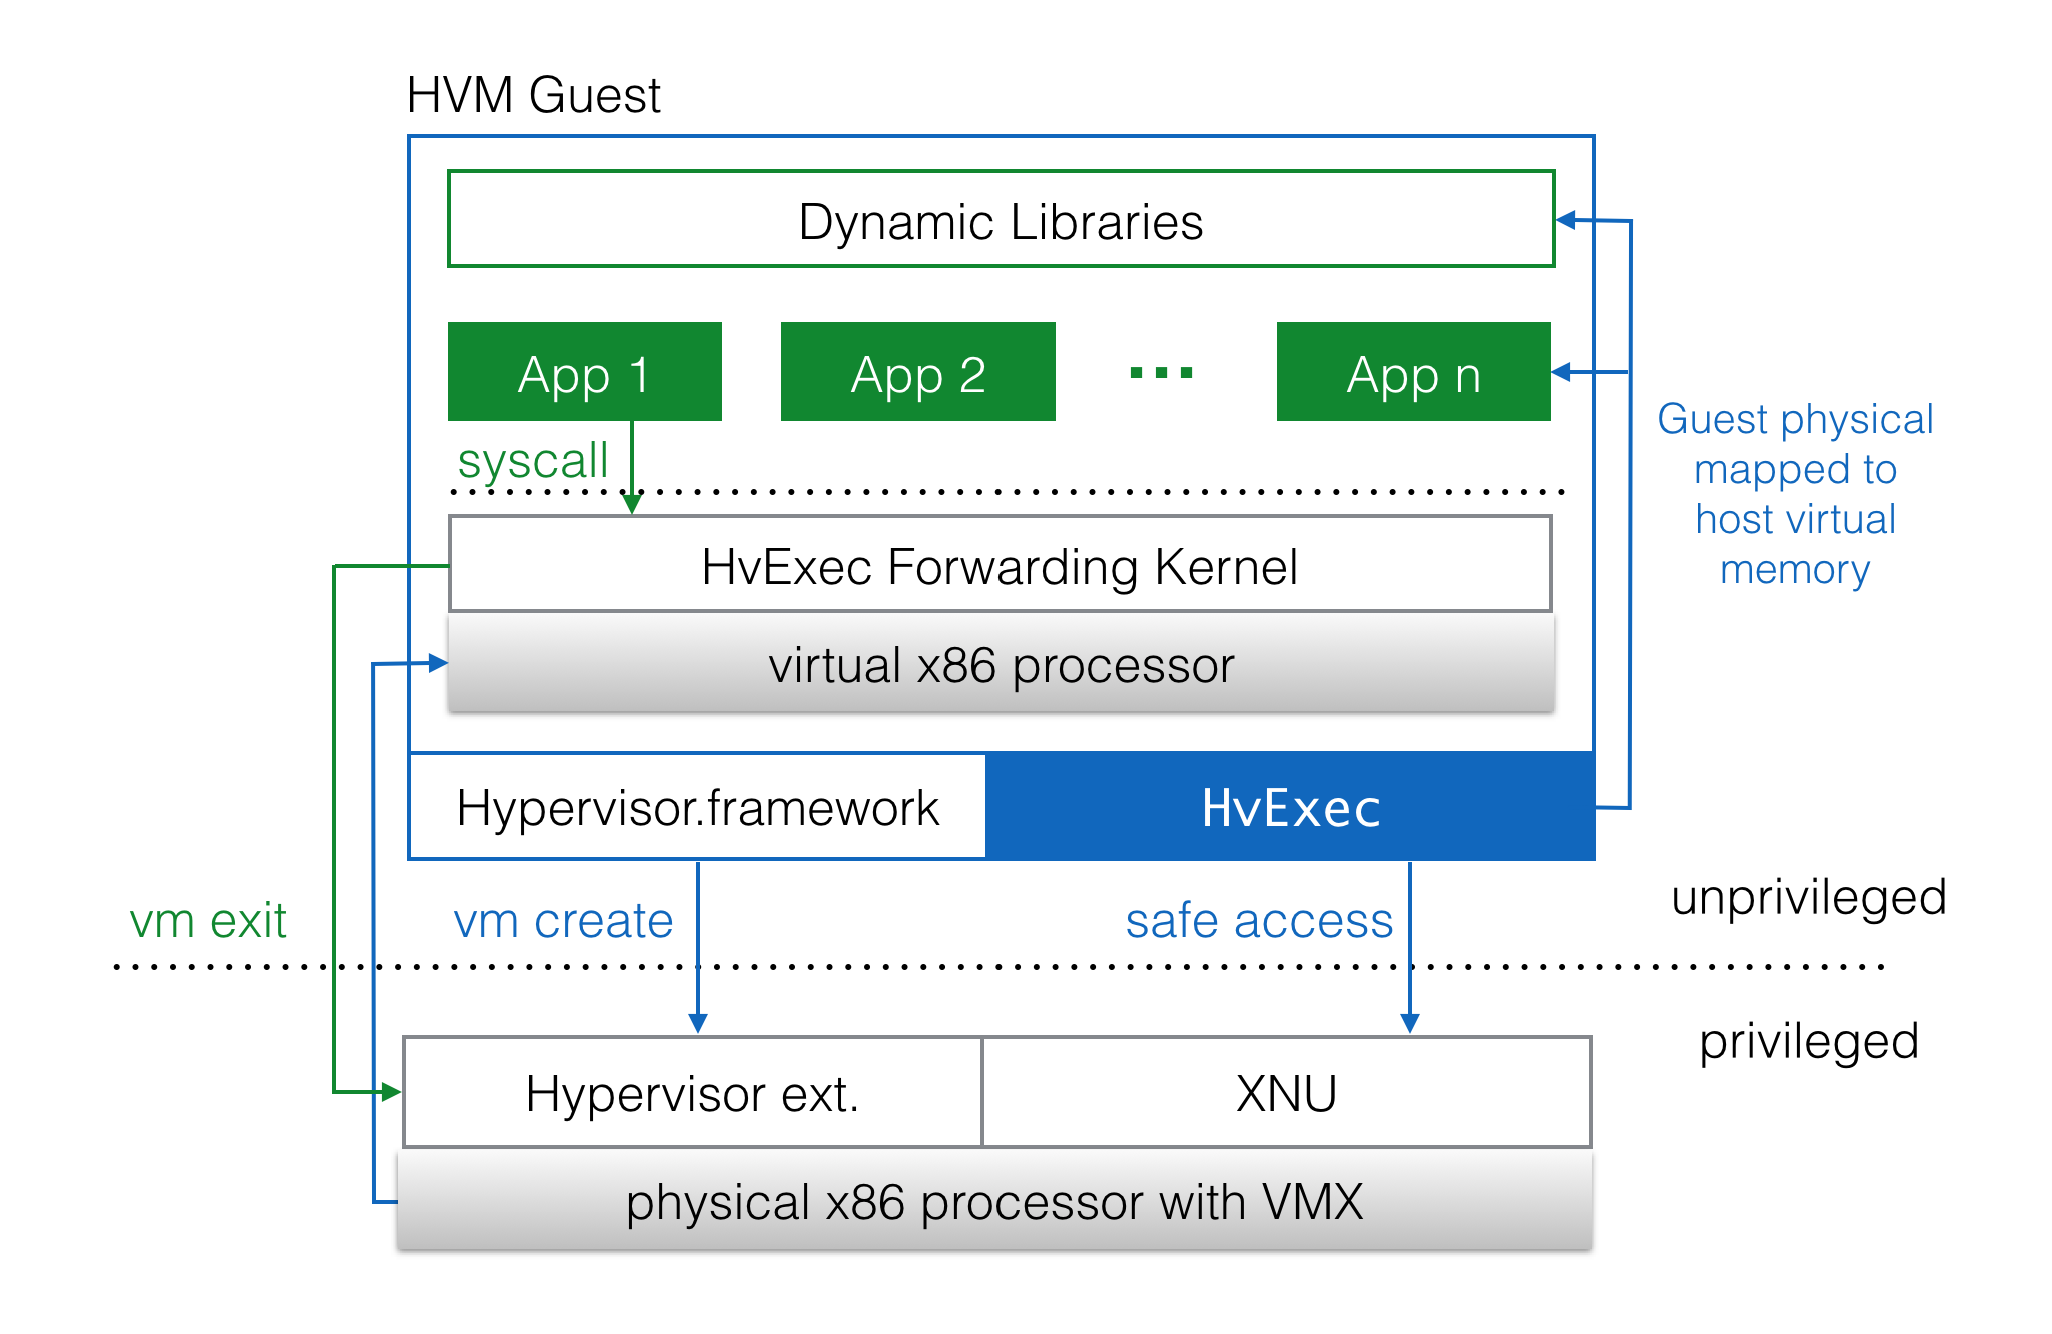
\includegraphics[width=16cm]{hvm}
    \caption{Diagram showing sandbox creation and system call interposition}
    \centering
\end{figure}
\subsection{Exitless Interrupts}
Context switching between host and guest is costly.
Describe a way to use shared memory between guest and host to implement a buffer queue for exitless
communication.
Method is similar to ones used in paravirtual IO drivers, but ultimately it uses a spin lock which might not be
power efficient.
When on low power or idle, switch back to context swtiching since applications running during this time will not likely to latency sensitive.
\subsection{System Call Emulation}
In short, how to accurately mirror the state of the host in the guest.
\subsection{Security}
How to avoid race conditions (time of check vs time of use) and guarantee sandbox cannot be circumvented.

\section{Implementation}
Virtualization hardware is widely deployed. Laptops, tablets and phones all processors with virtualization features.
We chose to build the prototype on OSX, a popular operating system among consumers and application writers in this era.
OSX has kernel support exposing the underlying x86 VT-x extensions through a system called Hypervisor.framework (analogous to KVM on Linux).
\subsection{Memory Management}
How to map memory into the guest and translate addresses from guest virtual to guest physical to host virtual to host physical.

With extended page tables (EPT), Intel added an Address Space Identifier (ASID) to
track which entry in the translation look aside buffer (TLB) belongs to which VM. Thus, context switching between
VMs don't necessarily flush the TLB.
\subsection{Dynamic Loader}
While some applications ship as single statically linked executable, most applications link against dynamic libraries.
It is the responsibility of the loader to map the dynamic libraries into the process address space and fill out the
symbol relocation tables.
\PROJNAME{} will also have to implement the loader functionality in order to run dynamically linked executables.
\subsection{Concurrency}
How to deal with fork() and threads? What about IPC?

\section{Evaluation}
Results for benchmarks.
\subsection{Context Switching Overhead}
Comparison between VMEXIT latency vs exitless approach.
\subsection{Scalability}
Performance degredation when scaling to hundreds of processes.

\section{Conclusions}
Summarize what was achieved and any room for improvement or problems unsolved.

\begin{itemize}
    \item
        Expands the capabilites of userspace and we hope to see virutalization being used outside of full OS virtualization.
    \item
        Foreign syscall emulation layer or compatiblity layer reducing burden on OS for maintaining binary compatible interfaces.
    \item
        Virtual application filesystems (more secure way to share resources).
        Think of it like a union filesystem per application.
    \item
        Better auditing.
    \item
        Address how debugging will work with sandbox.
    \item
        Two-way sandbox with SGX.
\end{itemize}

As we see server OSes being targeted for virtualization (hardware agnostic virtio drivers) maybe the same trend will appear for applications.
In the future, we may write applications against an OS agnositic "virtual syscall" interface.

\begin{thebibliography}{99}

\bibitem{DesignImplFreeBSD}
M. K. McKusick, G. V. Neville-Neil and R. N. M. Watson.
\emph{The Design and Implementation of the FreeBSD Operating System}.
Addison-Wesley Professional,
2nd edition,
2014.
ISBN-13: 978-0321968975.

\bibitem{Ostia2004}
T. Garfinkel, B. Pfaff and M. Rosenblum.
Ostia: A Delegating Architecture for Secure System Call Interposition.
\emph{NDSS, The Internet Society}, 2004.

\bibitem{VCall2010}
B. Li, J. Li, T. Wo, C. Hu and L. Zhong.
A VMM-based system call interposition framework for program monitoring.
In \emph{Parallel and Distributed Systems (ICPADS), 2010 IEEE 16th International Conference on}, 2010.

\bibitem{Ayer2012}
A. Ayer.
KVMSandbox: Application-Level Sandboxing with x86 Hardware Virtualization and KVM.
Master's Thesis, Brown University, 2012.

\bibitem{ELI2015}
N. Amit, A. Gordon, N. Har'El, M. Ben-Yehuda, A. Landau, A. Schuster and D. Tsafrir.
Bare-metal performance for virtual machines with exitless interrupts.
\emph{Communications of the ACM, 59}(1). 2015.

\bibitem{Ether2008}
A. Dinaburg, P. Royal, M. Sharif and W. Lee.
Ether: malware analysis via hardware virtualization extensions.
In \emph{Proceedings of the 15th ACM conference on Computer and communications security}.
ACM, 2008.
\end{thebibliography}

\iffalse
key advantages:
user API allows programmability.
runs arbitrary unmodified executables.
Compatible with conventional OS security.
Low latency and scales with multiprocessing.

Move from multi-user security to per application restrictions.
User level security is mature, but applications are too unrestricted.
Can access files without user consent and force consent by denying services.
Users don't ahve right tools. ACL permissions too coarse grained.
Existing policies are oriented towards restricing users not apps.
Controls are baked into the kernel making then risky to change.
Ultimately, we want to be able to run arbitrary binaries with assurances.

Least privileged operation

Others have tried to address this, but not address all problems completely.
Some existing work like SELinux, BSD Jails, BSD Capsicum aim to do application sandboxing.
Maybe good for servers but they dont provide the controls suitable for end users like fake resource masking.
Other prior work suffer from similar deficiencies as will explain in related work section.

Formed requirements based on lessons learned in the past and to address deficiencies.
List out the requirements:
unmodified binaries,
guarantee trap all system resource access,
avoid ways to circumvent policy agent,
safe (does not weaken existing security features, cannot circumvent existing security, works in addition to),
minimal/conservative kernel changes (minimize risk new bugs, no changes in critical code paths),
native performance (minimize context change overhead, scalability),
provide concrete implementation (often systems problems are not revealed until implemented)

Based on those requirements we think system call layer is the best place to interpose because it serves as a boundary between applications and all system resources.

Build a system call interposition layer in user-space using hardware virtualization (HVM) to monitor and regulate unmodified binaries.
Leverage HVM for isolation and guarantees traps.
Cite HVM good enough for malware containment.
VMs provides reliable isolation and guarantees privileged instructions are trapped.
Allows policy agent runs in memory isolated from untrusted application.
Leverages HVM extensions from OS virtualization but improves scalability and avoids duplicate work by not having to run a full guest OS.
Instructions in a VM are executed natively without any translation overhead
Don’t need to patch the kernel or install kernel modules for updates to support new features (leverage kernel support for HVM).
Better safety because host runs in unprivileged mode subject to existing OS security restrictions.
User controlled programmable security policies (updatable without kernel changes) like being able to deny access without revealing so by presenting fake resources to application.

What are the problems with syscall interposition sandboxes?
HVM alone does not guarantee security, also have to watch out for TOCTOU and other good practices.
Amortize context change overhead, but microbenchmarks indicate 22X overhead, furthermore investigate latency sensitive cases.
Cite VCall and Ayer thesis, maybe we can do better, latency not really investigated.
Investigate scalability (threading, multiprocessing) not addressed in prior work. One vm per process or put multiple processes in one vm? Scales to hundreds of processes?
Syscall transformation is novel feature not found in other sandboxes? Really important feature for privacy.

HVM is typically used in kernel virtualization but recently found use in less typical applications like malware analysis \cite{Ether2008} and sandboxing \cite{Ayer2012, VCall2010}.
Ether demonstates isolation and undetactability.
Most similar work include VCall and KVM sandbox to the best of our knowledge.
But they dont address scalability and syscall transformation.
Think of this a continuation for deeper investigation.
Ayer, beihan are closest implementations.
Ayer forks new process which simplifies implemenation but does not scale.
Beihan uses naive method of context switching not suitable for low latency applications.
Three categories of sandoxes. Focus on deficiencies in prior work.


\fi

\end{document}

